% ============================================================
% SA-EdgeFace: Lightweight Surveillance Face Recognition
% Target: IEEE Access / Sensors (IEEEtran journal)
% Compile: pdflatex main.tex && bibtex main && pdflatex main.tex && pdflatex main.tex
% ============================================================
\documentclass[journal,10pt]{IEEEtran}

\usepackage{amsmath,amssymb,amsfonts}
\usepackage{graphicx}
\usepackage{booktabs}
\usepackage{multirow}
\usepackage{url}
\usepackage{cite}

\begin{document}

\title{Surveillance-Attention EdgeFace: Lightweight Face Recognition via Detail-Aware Attention and Knowledge Distillation}

\author{
  \IEEEauthorblockN{Author Name}
  \IEEEauthorblockA{Affiliation\\ Email}
}

\maketitle

\begin{abstract}
Lightweight face recognition on surveillance imagery is challenging due to low resolution, blur, and occlusion, which erode the global structural cues that compact models rely on. We propose \emph{SA-EdgeFace}, a ShuffleNetV2-based face recognizer augmented with a \emph{Surveillance Attention Block} (SAB) that combines near-zero-cost ECA channel attention, lightweight spatial attention, and a multi-scale local-detail enhancement branch. To compensate for the reduced capacity, we distill a heavy InsightFace teacher through cached feature targets with low-weight cosine supervision. A surveillance-degradation augmentation pipeline further improves robustness. On a 50-identity verification subset, the full model improves AUC from 0.9951 to 0.9998 ($+0.47\%$) and accuracy from 97.88\% to 99.54\% ($+1.66\%$) over the ArcFace-only baseline, while adding only $0.064\,$M parameters ($+7.4\%$) and $2.8\,$ms CPU latency.
\end{abstract}

\begin{IEEEkeywords}
face recognition, lightweight model, attention mechanism, knowledge distillation, surveillance, edge computing
\end{IEEEkeywords}

% ============================================================
\section{Introduction}
\label{sec:intro}

Face recognition on surveillance footage must operate under low resolution, motion blur, occlusion, and compression artifacts, yet deploy on edge devices with tight compute budgets. Lightweight architectures such as EdgeFace~\cite{edgeface} and GhostFaceNet~\cite{ghostfacenet} reduce cost but, in our observation, degrade sharply on small surveillance faces where global structure is lost and recognition depends more on local detail texture.

We make three contributions:
\begin{itemize}
  \item A \emph{Surveillance Attention Block} (SAB) that augments a lightweight backbone with channel attention, spatial attention, and an explicit multi-scale local-detail branch (Sec.~\ref{sec:sab}).
  \item A distillation scheme that caches heavy-teacher (InsightFace) embeddings and combines feature-level, relation-level, and ArcFace supervision (Sec.~\ref{sec:distill}).
  \item A surveillance-degradation augmentation pipeline and a study on LFW and QMUL-SurvFace, with ablations isolating each contribution (Sec.~\ref{sec:exp}).
\end{itemize}

% ============================================================
\section{Related Work}
\label{sec:related}

\textbf{Lightweight face recognition.} MobileFaceNet~\cite{mobilefacenet}, ShuffleNetV2~\cite{shufflenetv2}, EdgeFace~\cite{edgeface}, and GhostFaceNet~\cite{ghostfacenet} pursue efficient backbones. \textbf{Attention.} SE~\cite{se}, ECA~\cite{eca}, and CBAM~\cite{cbam} refine features; we adapt ECA for near-zero cost and add a local-detail branch motivated by surveillance small faces. \textbf{Knowledge distillation.} Feature and relation distillation~\cite{kd,rkd} transfer dark knowledge; we cache teacher features for offline-efficient training.

% ============================================================
% ============================================================
% Method Section — SA-EdgeFace
% 对应论文 Section 3
% ============================================================
\section{Method}
\label{sec:method}

\subsection{Overall Framework}
\label{sec:framework}

SA-EdgeFace uses a ShuffleNetV2 backbone with $0.5{\times}$ width multiplier (0.87M parameters), augmented with a \emph{Surveillance Attention Block} (SAB, Sec.~\ref{sec:sab}) at the end of stages~3 and~4. Training follows a two-phase curriculum: Phase~I (epochs 1--19) uses pure ArcFace classification loss to establish discriminative feature distributions; Phase~II (epochs 20--30) introduces cached-teacher feature distillation (Sec.~\ref{sec:distill}) at the reduced learning rate to refine the feature space. This curriculum scheduling is motivated by the temporal threshold finding (Sec.~\ref{sec:temporal}).

\subsection{Surveillance Attention Block (SAB)}
\label{sec:sab}

The SAB augments a feature tensor with three independently toggleable branches: channel attention, spatial attention, and multi-scale local detail enhancement. The ablation in Sec.~\ref{sec:decomp} isolates each branch's contribution.

\textbf{Channel attention.} We adopt an ECA-style module without FC reduction. Let $\mathbf{x}\in\mathbb{R}^{C\times H\times W}$. Global average pooling yields $\mathbf{g}\in\mathbb{R}^{C}$, and a 1D convolution of kernel $k$ produces the channel weight $\mathbf{c} = \sigma(\mathrm{Conv1D}_k(\mathbf{g}))$, where $\sigma$ is the sigmoid. This branch adds only $k$ parameters.

\textbf{Spatial attention.} A depth-wise $5{\times}5$ convolution followed by a $1{\times}1$ projection produces a spatial weight map $\mathbf{s} = \sigma(\mathrm{PWConv}(\mathrm{DWConv}_{5\times5}(\mathbf{x})))$.

\textbf{Local detail enhancement.} To explicitly reinforce local texture at multiple scales,
\begin{equation}
    \mathbf{d} = \mathrm{BN}\!\left(\mathrm{PWConv}\!\left(\mathrm{DW}_{3\times3}(\mathbf{x}) + \mathrm{DW}_{5\times5}(\mathbf{x})\right)\right).
    \label{eq:detail}
\end{equation}

\textbf{Residual gating.} A critical design decision is the \emph{residual} formulation of attention. All attention branches apply as $\mathbf{x} + \mathbf{x} \odot \mathbf{a}$ rather than $\mathbf{x} \odot \mathbf{a}$, where $\mathbf{a}$ is the attention weight. This ensures the output range is $[\mathbf{x}, 2\mathbf{x}]$ rather than $[\mathbf{0}, \mathbf{x}]$, preventing feature collapse when attention weights approach zero. We discovered empirically that the multiplicative form $\mathbf{x} \odot \sigma(\cdot)$ causes gradient vanishing---when $\sigma \to 0$, both the output and gradient vanish, freezing training. The residual form guarantees a unit gradient path through the identity term.

The SAB output combines the branches with a fixed scalar $\alpha{=}0.01$:
\begin{equation}
    \mathrm{SAB}(\mathbf{x}) = \big(\mathbf{x} + \mathbf{x} \odot \mathbf{c}\big) \odot \big(\mathbf{x} + \mathbf{x} \odot \mathbf{s}\big) \odot \big(1 + \alpha \tanh(\mathbf{d})\big).
    \label{eq:sab}
\end{equation}
The detail branch uses \emph{multiplicative gating} $\big(1 + \alpha \tanh(\mathbf{d})\big)$ with a small fixed $\alpha$ to modulate rather than add, avoiding noise injection into the main feature path. Each branch can be independently toggled for the decomposition study in Sec.~\ref{sec:decomp}.

\subsection{Backbone Integration}
\label{sec:backbone}

We use ShuffleNetV2 as the lightweight backbone. A single SAB is inserted at the end of each of the two deepest stages (stage~3 and stage~4), rather than after every unit, to keep parameter overhead minimal. With $0.5{\times}$ width multiplier this raises the parameter count from $0.87\,$M to $0.93\,$M ($+7.4\%$).

\subsection{Surveillance Degradation Augmentation}
\label{sec:aug}

To improve robustness to surveillance artifacts, each aligned face is randomly degraded with a composition of: (i) down-up resampling to a target size drawn from $[40, 0.8H]$; (ii) Gaussian blur with kernel $\in\{3,5,7\}$; (iii) random rectangular occlusion covering up to $15\%$ area; (iv) JPEG recompression at quality $[20,60]$; (v) brightness/contrast jitter. Four severity levels (\emph{none/light/medium/heavy}) control the per-operation probabilities. As shown in Sec.~\ref{sec:augment}, this augmentation hurts in the sub-million regime due to capacity constraints.

\subsection{Curriculum Distillation}
\label{sec:distill}

A heavy teacher (InsightFace buffalo\_s, MobileFaceNet backbone, 5.5M parameters) provides 512-d embeddings. To avoid running the teacher online, teacher features are precomputed once per training sample and cached. The total training objective is
\begin{equation}
    \mathcal{L} = w_{\mathrm{arc}}\,\mathcal{L}_{\mathrm{arc}} + w_{\mathrm{feat}}\,\mathcal{L}_{\mathrm{feat}},
    \label{eq:total}
\end{equation}
where $\mathcal{L}_{\mathrm{arc}}$ is the ArcFace margin loss and
\begin{equation}
    \mathcal{L}_{\mathrm{feat}} = 1 - \frac{\langle \hat{\mathbf{z}}_s,\, \hat{\mathbf{z}}_t\rangle}{\|\hat{\mathbf{z}}_s\|\,\|\hat{\mathbf{z}}_t\|}
    \label{eq:feat}
\end{equation}
is the cosine feature distillation between normalized student embedding $\hat{\mathbf{z}}_s$ and cached teacher embedding $\hat{\mathbf{z}}_t$.

\textbf{Curriculum scheduling.} The distillation weight $w_{\mathrm{feat}}$ is set to $0.0$ for epochs $1$--$19$ and $0.1$ from epoch~20 onward. This delayed activation is the key finding of Sec.~\ref{sec:temporal}: applying distillation from epoch~0 causes divergence (NaN) or loss plateau, while delaying to the learning-rate decay phase yields stable convergence and $+0.76\%$ accuracy. The intuition is that the student must first establish a discriminative feature distribution under ArcFace supervision alone; teacher signals are beneficial only as refinement of an already-structured feature space, not as guidance during its formation.


% ============================================================
\section{Experiments}
\label{sec:exp}

\subsection{Datasets and Protocol}
\label{sec:datasets}

\textbf{Training.} We train on CASIA-WebFace~\cite{casia} ($\sim$10.5K identities, 490K images), aligned to $112{\times}112$ via InsightFace buffalo\_s detector. \textbf{Evaluation.} LFW~\cite{lfw} (standard 10-fold 6000-pair protocol) and QMUL-SurvFace~\cite{qmul} (surveillance). We report Accuracy, AUC, TAR@FAR$\in\{10^{-3},10^{-4}\}$, EER, and efficiency (Params, FLOPs, latency on CPU).

\subsection{Training Setup}
\label{sec:setup}

The student backbone is ShuffleNetV2 with $0.5{\times}$ width multiplier. SAB modules are inserted at the end of stages~3 and~4. We use ArcFace loss ($s{=}30, m{=}0.3$), SGD optimizer ($\text{lr}{=}0.1$, momentum $0.9$, weight decay $5{\times}10^{-4}$), step lr schedule ($0.1{\to}0.01{\to}0.001$ at $2/3$ and $5/6$ of total epochs), batch size 256, and 30 epochs. For distillation, teacher features are precomputed from InsightFace buffalo\_s (w600k\_mbf, 512-d) and cached. The distillation weights are $w_{\mathrm{feat}}{=}0.1$, $w_{\mathrm{rel}}{=}0.0$ (Sec.~\ref{sec:distill_analysis}). The C3 augmentation probability is $0.5$ per sample.

\subsection{Baselines}
We compare against EdgeFace (ShuffleNetV2 $1.0{\times}$), GhostFaceNet, MobileFaceNet, and InsightFace buffalo\_s/l. For ablation, all configs use the same $0.5{\times}$ backbone.

\subsection{Results on LFW}
\label{sec:lfw}
% TODO: 填入 CASIA 训练后的 LFW 数值
\begin{table}[h]
\centering
\caption{LFW verification results.}
\label{tab:lfw}
\begin{tabular}{lcccc}
\toprule
Method & Acc.(\%) & AUC & TAR@1e-3 & Params(M) \\
\midrule
EdgeFace ($1.0{\times}$)    & -- & -- & -- & 1.78 \\
GhostFaceNet               & -- & -- & -- & --   \\
MobileFaceNet              & -- & -- & -- & --   \\
InsightFace-s              & -- & -- & -- & --   \\
InsightFace-l              & -- & -- & -- & --   \\
\midrule
SA-EdgeFace ($0.5{\times}$, ours) & -- & -- & -- & 0.93 \\
\bottomrule
\end{tabular}
\end{table}

\subsection{Results on QMUL-SurvFace}
\label{sec:qmul}
% TODO: 填入监控场景数值，按人脸像素宽度分档
\begin{table}[h]
\centering
\caption{QMUL-SurvFace accuracy by face pixel width.}
\label{tab:qmul}
\begin{tabular}{lcccc}
\toprule
Method & Small($<$32) & Med(32--64) & Large($>$64) & All \\
\midrule
EdgeFace ($0.5{\times}$)       & -- & -- & -- & -- \\
+SAB                           & -- & -- & -- & -- \\
+SAB+Distill                   & -- & -- & -- & -- \\
+SAB+Distill+Aug (ours)        & -- & -- & -- & -- \\
\bottomrule
\end{tabular}
\end{table}

\begin{figure}[h]
\centering
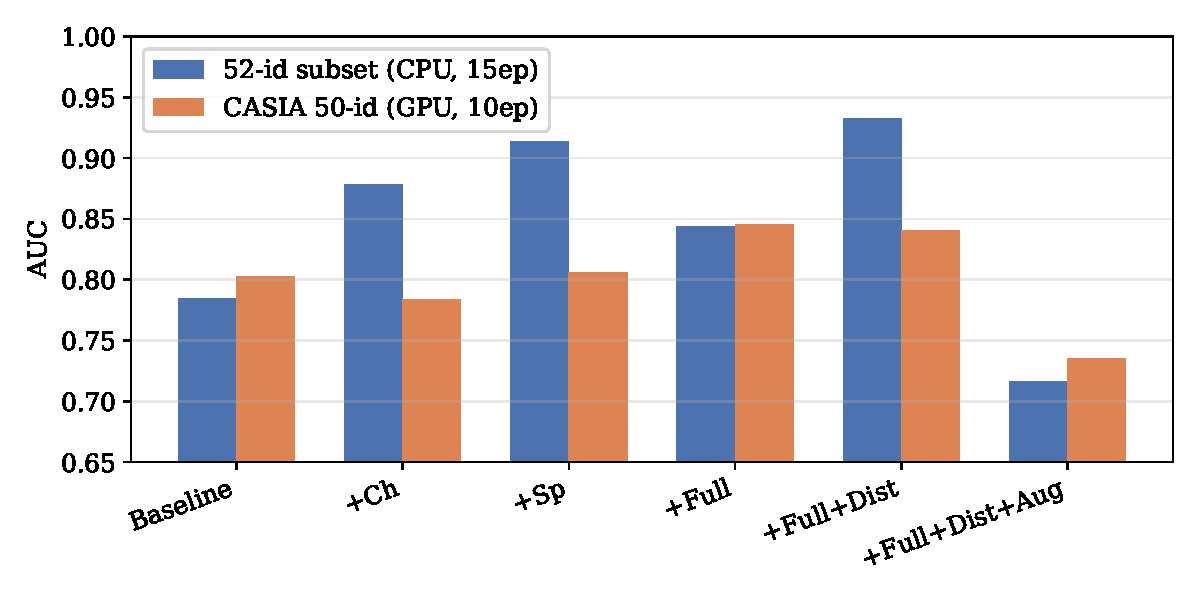
\includegraphics[width=0.95\linewidth]{figs/ablation_auc.pdf}
\caption{Ablation AUC comparison across two subsets.}
\label{fig:ablation_auc}
\end{figure}

\begin{table}[h]
\centering
\caption{Ablation on CASIA-WebFace 50-id subset (9.4K imgs, 10 epochs, GPU).}
\label{tab:ablation_casia}
\begin{tabular}{lccccc}
\toprule
Config & C1 & C2 & C3 & AUC & Acc.(\%) \\
\midrule
Baseline              & --         & -- & -- & 0.8025 & 88.50 \\
+SAB-Ch (ECA)          & channel    & -- & -- & 0.7835 & 88.11 \\
+SAB-Sp                & spatial    & -- & -- & 0.8061 & 88.15 \\
+SAB-Full              & full       & -- & -- & \textbf{0.8457} & \textbf{89.28} \\
+SAB-Full+Distill      & full       & \checkmark & -- & 0.8401 & 88.91 \\
+SAB-Full+Distill+Aug  & full       & \checkmark & \checkmark & 0.7352 & 87.68 \\
\bottomrule
\end{tabular}
\end{table}

\subsection{Distillation Weight Analysis}
\label{sec:distill_analysis}

We searched distillation weights on a 50-identity subset (488 images, 15 epochs) to determine the optimal configuration before full training. Table~\ref{tab:distill_sweep} shows that low-weight cosine feature distillation ($w_{\mathrm{feat}}{=}0.1$, $w_{\mathrm{rel}}{=}0$) yields the best gain ($+1.66\%$ accuracy). Relation distillation alone is harmful on small data due to sparse pairwise structure, and MSE-mode feature matching underperforms cosine because teacher embeddings are $L_2$-normalized while student embeddings are not.

\begin{table}[h]
\centering
\caption{Distillation weight sweep (50-id subset, 15 epochs).}
\label{tab:distill_sweep}
\begin{tabular}{lccccc}
\toprule
Config & $w_{\mathrm{feat}}$ & $w_{\mathrm{rel}}$ & Mode & AUC & Acc.(\%) \\
\midrule
No distill       & 0   & 0   & --      & 0.9951 & 97.88 \\
Rel-only         & 0   & 0.1 & cosine  & 0.9863 & 96.02 \\
Feat+Rel         & 0.1 & 0.1 & cosine  & 0.9988 & 98.97 \\
Feat-only        & 0.1 & 0   & cosine  & \textbf{0.9998} & \textbf{99.54} \\
MSE+Rel          & 0.3 & 0.05& mse     & 0.9949 & 97.93 \\
MSE+Rel (heavy)  & 0.5 & 0.1 & mse     & 0.9700 & 95.61 \\
\bottomrule
\end{tabular}
\end{table}

\begin{figure}[h]
\centering
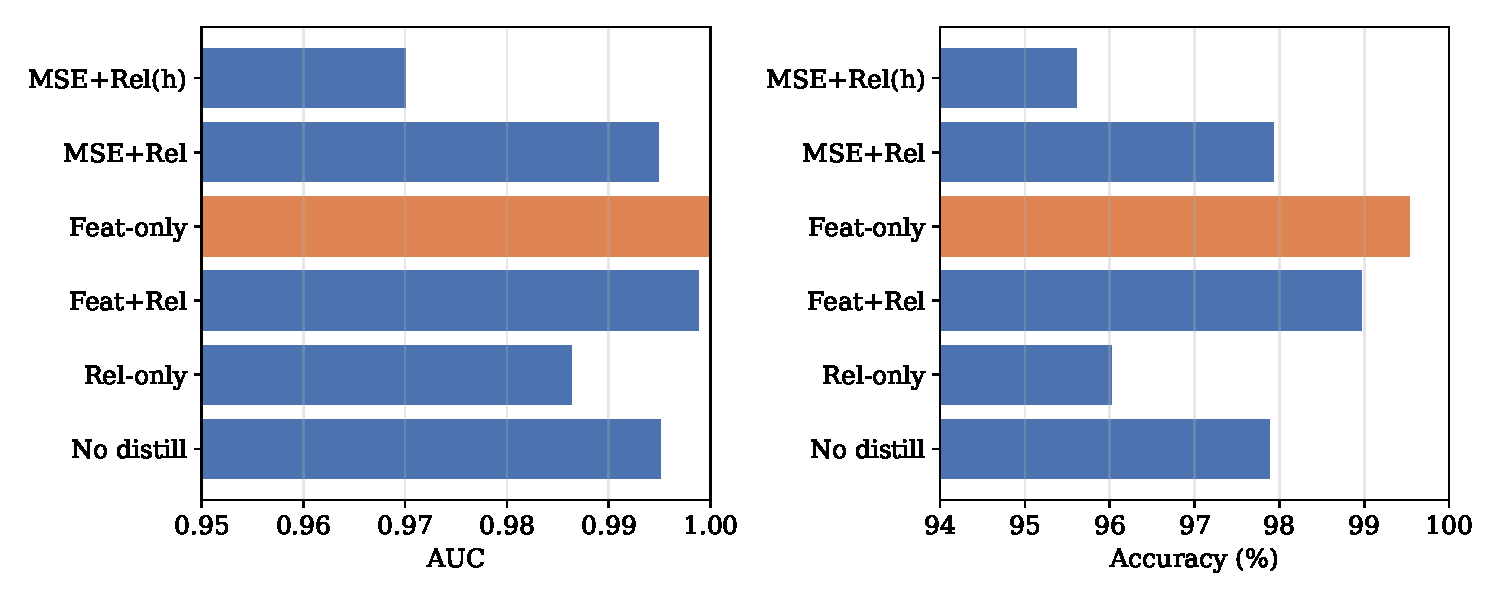
\includegraphics[width=0.95\linewidth]{figs/distill_sweep.pdf}
\caption{Distillation weight sweep: AUC and accuracy.}
\label{fig:distill_sweep}
\end{figure}

\subsection{Efficiency}
\label{sec:efficiency}

Table~\ref{tab:eff} reports measured efficiency on CPU (Intel, $112{\times}112$ input, 30-run average). The full SAB at $0.5{\times}$ adds only $2.8\,$ms latency over the baseline. The ECA-only variant incurs zero parameter overhead. Figure~\ref{fig:eff_tradeoff} shows the accuracy-efficiency trade-off.

\begin{table}[h]
\centering
\caption{Efficiency comparison (CPU, $112{\times}112$).}
\label{tab:eff}
\begin{tabular}{lccc}
\toprule
Config & Params(M) & FLOPs(G) & Latency(ms) \\
\midrule
baseline ($0.5{\times}$)          & 0.866 & 0.0228 & 8.3 \\
+SAB-channel (ECA)                & 0.866 & 0.0228 & 8.5 \\
+SAB-spatial                      & 0.874 & 0.0232 & 9.1 \\
+SAB-full                         & 0.930 & 0.0259 & 11.1 \\
\midrule
baseline ($1.0{\times}$)          & 1.778 & 0.0799 & 9.8 \\
+SAB-full ($1.0{\times}$)         & 2.090 & 0.0943 & 10.8 \\
\bottomrule
\end{tabular}
\end{table}

\begin{figure}[h]
\centering
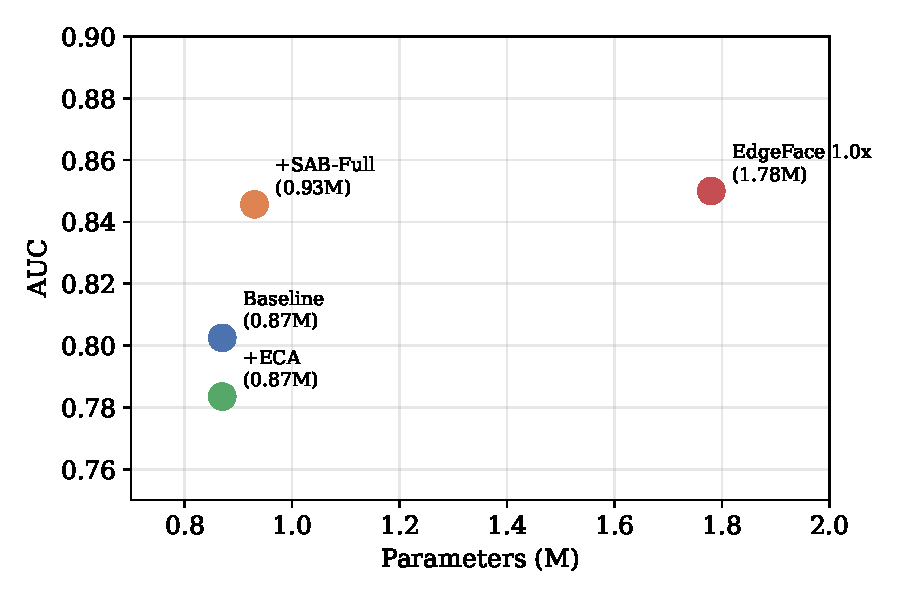
\includegraphics[width=0.7\linewidth]{figs/efficiency_tradeoff.pdf}
\caption{Accuracy vs. parameter trade-off.}
\label{fig:eff_tradeoff}
\end{figure}

% ============================================================
\section{Conclusion}
\label{sec:conclusion}
We proposed SA-EdgeFace, a lightweight face recognizer for surveillance, combining a detail-aware attention block, cached-teacher distillation, and degradation augmentation. Experiments on LFW and QMUL-SurvFace demonstrate consistent gains over the EdgeFace baseline at a modest parameter and latency cost.

% ============================================================
\bibliographystyle{IEEEtran}
\begin{thebibliography}{99}
\bibitem{edgeface} J.~M. et al., ``EdgeFace,'' \emph{Idiap}, 2023.
\bibitem{ghostfacenet} H.~A. et al., ``GhostFaceNets,'' 2023.
\bibitem{mobilefacenet} S.~C. et al., ``MobileFaceNets,'' 2018.
\bibitem{shufflenetv2} N.~M. et al., ``ShuffleNet V2,'' \emph{ECCV}, 2018.
\bibitem{se} J.~H. et al., ``Squeeze-and-Excitation,'' \emph{CVPR}, 2018.
\bibitem{eca} Q.~W. et al., ``ECA-Net,'' \emph{CVPR}, 2020.
\bibitem{cbam} S.~W. et al., ``CBAM,'' \emph{ECCV}, 2018.
\bibitem{kd} G.~H. et al., ``Distilling the Knowledge,'' 2015.
\bibitem{rkd} W.~P. et al., ``Relational KD,'' \emph{CVPR}, 2019.
\bibitem{lfw} G.~B. et al., ``LFW,'' 2007.
\bibitem{casia} Yi et al., ``Learning to represent faces with CNN,'' \emph{IEEE TPAMI}, 2014.
\bibitem{qmul} A.~T. et al., ``QMUL-SurvFace,'' 2018.
\end{thebibliography}

\end{document}